\documentclass[a4paper,12pt]{report}

% Page layout
\usepackage[left=2.5cm,right=2.5cm,top=2.5cm,bottom=2.5cm]{geometry}

% Font and text
\usepackage[afrikaans,english]{babel}
\usepackage{microtype}
\usepackage{setspace}
\usepackage{lmodern}
\usepackage{siunitx}
\newcommand{\myemph}[1]{{\sffamily\bfseries#1}}
\sloppy
\onehalfspacing

% Headings
\usepackage[raggedright,sf,bf]{titlesec}
\usepackage[margin=\the\parindent,small,bf,sf]{caption}
\titlelabel{\thetitle.\ }
\titleformat{\chapter}[display]{\huge\bfseries\sffamily}{\chaptertitlename\ \thechapter}{15pt}{\Huge \raggedright}
\titlespacing*{\chapter}{0pt}{0pt}{40pt}  % remove spacing before chapter headings
\makeatletter
\let\originall@chapter\l@chapter
\def\l@chapter#1#2{\originall@chapter{{\sffamily #1}}{#2}}
\makeatother

%% Alternative headings using small-caps (comment out the top section)
%\usepackage[raggedright,bf]{titlesec}
%\usepackage[margin=\the\parindent,small,bf]{caption}
%\titlelabel{\thetitle.\ }
%\titleformat{\chapter}[display]{\huge\scshape}{\chaptertitlename\ \thechapter}{15pt}{\Huge \raggedright}
%\titlespacing*{\chapter}{0pt}{0pt}{40pt}  % remove spacing before chapter headings

% Table of contents
\let \savenumberline \numberline
\def \numberline#1{\savenumberline{#1.}}

% Figures
\usepackage{graphicx}
\usepackage{pdfpages}
\usepackage{subcaption}
\setlength{\abovecaptionskip}{7.5pt}  % spacing above and below captions
\newcommand*{\WaterMark}[2][0.2\paperwidth]{\AddToShipoutPicture*{\AtTextCenter{\parbox[c]{0pt}{\makebox[0pt][c]{\includegraphics[width=#1]{#2}}}}}}

% Mathematics
\usepackage[cmex10]{amsmath}
\usepackage{amssymb}
\usepackage{cancel}
\DeclareMathOperator*{\argmax}{arg\,max}
\newcommand{\T}{^\top}
\newcommand{\tr}{\textrm{tr}}
\renewcommand{\vec}[1]{\boldsymbol{\mathbf{#1}}}
\newcommand{\defeq}{\triangleq}

% Tables
\usepackage{booktabs}
\usepackage{tabularx}
\usepackage{multirow}
\newcommand{\mytable}{
    \centering
    \small
    \renewcommand{\arraystretch}{1.2}
    }
\renewcommand{\tabularxcolumn}[1]{m{#1}}
\newcolumntype{C}{>{\centering\arraybackslash}X}
\newcolumntype{L}{>{\raggedright\arraybackslash}X}

% Header and footer
\usepackage{fancyhdr}
\pagestyle{fancy}
\fancyhf{}
\renewcommand{\sectionmark}[1]{\markright{\normalsize \thesection.\ #1}}
\fancyhead[C]{\nouppercase{\textit{\rightmark}}}
\fancyhead[RO]{\thepage}
 \fancyhead[LE]{\thepage}  % double-sided printing
\fancyfoot{}
\setlength\headheight{14.5pt}
\renewcommand{\headrulewidth}{0pt}
\fancypagestyle{plain}{\fancyhead{}
                       \renewcommand{\headrulewidth}{0pt}
                       \fancyfoot[C]{\thepage}}

% Pseudo-code
\usepackage{algorithm}  % should go before \usepackage{hyperref}

% Table of contents and hyperlinks
\usepackage{hyperref}
\hypersetup{colorlinks=true,linktoc=all,citecolor=black,linkcolor=black}
\usepackage[nottoc]{tocbibind}

% Pseudo-code
\usepackage{algpseudocode}  % should go after \usepackage{hyperref}
\renewcommand{\thealgorithm}{\arabic{chapter}.\arabic{algorithm}} 
\captionsetup[algorithm]{labelfont={bf,sf},font=small,labelsep=colon}

% Bibliography
\usepackage{cite}  % automatically reorder inline citations
\bibliographystyle{IEEEtran}

% Fix titlesec issue
\usepackage{etoolbox}
\makeatletter
\patchcmd{\ttlh@hang}{\parindent\z@}{\parindent\z@\leavevmode}{}{}
\patchcmd{\ttlh@hang}{\noindent}{}{}{}
\makeatother


\begin{document}

% Front matter
\graphicspath{{frontmatter/fig/}}
\pagenumbering{Alph}

\begin{titlepage}
	\begin{center}
		
		
\includegraphics[width=10cm]{US}
		
		\vfill
		
		{\sffamily \bfseries \huge Development of a tool for the extraction of low frequency mean square flux noise figures in SQUIDs \par}
%		{\scshape \huge A Critical Analysis of Design Flaws in the Death Star \par}
		
		\vfill
		
		{\large {\Large Paul Rossouw} \\ 23572027 \par}
		
		\vfill
		
		\vfill
		
		{Report submitted in partial fulfilment of the requirements of the module \\
			Project (E) 448 for the degree Baccalaureus in Engineering in the Department of
			Electrical and Electronic Engineering at Stellenbosch University. \par}
		
		\vfill
		
		{\large {Supervisor}: Prof C.\ J.\ Fourie} %\\
		% Department of Electrical and Electronic Engineering \par}
		
		\vfill
		
		{\Large October 2023}
	\end{center}
\end{titlepage}

%\graphicspath{{frontmatter/fig/}}
\pagenumbering{Alph}

\begin{titlepage}
	\begin{center}
		
		%
\includegraphics[width=10cm]{USlogo-top}
		
		\WaterMark{UScrest-WM}
		
		~\vspace{4.5em}
		
		{\sffamily \bfseries \huge A Critical Analysis of Design Flaws in the Death Star \par}
%		{\scshape \huge A Critical Analysis of Design Flaws in the Death Star \par}		
		
		\vspace{7em}
		
		{\large {\Large  Luke Skywalker} \\ 99652154 \par}
		
		\vspace{8em}
		
		{\large Thesis presented in partial fulfilment of the requirements for the degree of \\ Master of Engineering (Electronic) in the Faculty of Engineering at Stellenbosch University. \par}
		
		\vfill
		
		{\large {Supervisor}: Dr O.\ W.\ Kenobi\\
		Department of Electrical and Electronic Engineering \par}
		
		%\vfill
		\vspace{10em}
		
		{\Large October 2099}
	\end{center}
\end{titlepage}

\pagenumbering{roman}
\chapter*{Acknowledgements}
% \addcontentsline{toc}{chapter}{Acknowledgements}
\makeatletter\@mkboth{}{Acknowledgements}\makeatother

Firstly I would like to thank my parents for their unconditional love and support. They have made this journey possible. I would also like to thank my brother and sister for always challenging me. Lastly, I would like to thank my oupa Dawie for inspiring me to pursue a technical degree. 
%\chapter*{Declaration}
\newpage
\thispagestyle{plain}
\addcontentsline{toc}{chapter}{Declaration}
\makeatletter\@mkboth{}{Declaration}\makeatother

\centerline{
\includegraphics[width=8cm]{USlogo-top}}
\vspace*{-10pt}

\section*{\centering Plagiaatverklaring / \textit{Plagiarism Declaration}}

\vspace*{5pt}

\begin{enumerate}
    \item Plagiaat is die oorneem en gebruik van die idees, materiaal en ander intellektuele eiendom van ander persone asof dit jou eie werk is.\\
    \textit{Plagiarism is the use of ideas, material and other intellectual property of another's work
        and to present is as my own.}
    
    \item Ek erken dat die pleeg van plagiaat 'n strafbare oortreding is aangesien dit 'n vorm van diefstal is.\\
    \textit{I agree that plagiarism is a punishable offence because it constitutes theft.}
    
    \item Ek verstaan ook dat direkte vertalings plagiaat is. \\
    \textit{I also understand that direct translations are plagiarism.}
    
    \item Dienooreenkomstig is alle aanhalings en bydraes vanuit enige bron (ingesluit die internet) volledig verwys (erken). Ek erken dat die woordelikse aanhaal van teks sonder aanhalingstekens (selfs al word die bron volledig erken) plagiaat is. \\
    \textit{Accordingly all quotations and contributions from any source whatsoever (including the internet) have been cited fully. I understand that the reproduction of text without quotation marks (even when the source is cited) is plagiarism}
    
    \item Ek verklaar dat die werk in hierdie skryfstuk vervat, behalwe waar anders aangedui, my eie oorspronklike werk is en dat ek dit nie vantevore in die geheel of gedeeltelik ingehandig het vir bepunting in hierdie module/werkstuk of 'n ander module/werkstuk~nie. \\
    \textit{I declare that the work contained in this assignment, except where otherwise stated, is my original work and that I have not previously (in its entirety or in part) submitted it for grading in this module/assignment or another module/assignment.}
\end{enumerate}

\vfill

\noindent \begin{tabularx}{1.0\linewidth}{|L|L|}
    \hline
    \vspace{1cm} {Studentenommer / \textit{Student number}} & \vspace{1cm} {Handtekening / \textit{Signature}} \\
    \hline
    \vspace{1cm} {Voorletters en van / \textit{Initials and surname}} & \vspace{1cm} {Datum / \textit{Date}} \\
    \hline
\end{tabularx}

\vspace{15pt}

% The old declaration

%I, the undersigned, hereby declare that the work contained in this report is my own original work unless otherwise stated.
%
%% Afrikaans:
%% Hiermee verklaar ek, die ondergetekende, dat die werk in hierdie verslag vervat my eie oorspronklike werk is, tensy anders vermeld.
%
%\vspace{2.5cm}
%
%\begin{table}[h]
%\begin{tabular}{@{}p{2.5cm}p{5cm}}
%    Signature: & \dotfill \\
%    & \multicolumn{1}{c}{Obi-Wan Kenobi} \\
%    ~\vspace{1cm} \\
%    Date: & \dotfill \\
%\end{tabular}
%\end{table}
%
%\vfill
%
%\begin{center}
%    Copyright \textcopyright\ 2099 Stellenbosch University \\
%    All rights reserved
%\end{center}


\chapter*{Abstract}
\addcontentsline{toc}{chapter}{Abstract}
\makeatletter\@mkboth{}{Abstract}\makeatother

\subsubsection*{English}

The phenomenon of 1/f flux noise in superconducting quantum interference devices (SQUIDs) is known to be the limiting factor in the performance of biomagnetic sensors and qubits. In this project a numerical framework for calculating the mean square flux noise (MSFN) figure for an arbitrary SQUID design is implemented. The implementation aims to be flexible such that changes in the numerical framework does not require significant changes in the implementation. The project demonstrates how InductEx can be used for this purpose. It further describes the design and implementation of an optimisation technique. Results show that the model for the 1/f noise chosen is not correct but still has potential as a useful tool for design. The optimisation technique shows promising results and can speed up computation time by a factor of 180 while introducing a maximum error of $8\%$. Recent studies suggest more sophisticated models that are extensions of the model assumed in the derivation of the numerical framework. These models could potentially be implemented by extending the implementation presented in this project.

\selectlanguage{afrikaans}

\subsubsection*{Afrikaans}

Die verskynsel van 1/f  magnetiese vloed steurings in superconducting quantum interference devices (SQUIDs) is bekend as die beperkende faktor in die ontwikkeling van beter biomagnetiese sensore en qubits. In hierdie projek word 'n numeriese raamwerk geïmplementeer om die gemiddelde kwadraat magnetiese vloed steurings (MSFN) waarde vir 'n willekeurige SQUID-ontwerp te bereken. Die implementasie streef daarna om aanpasbaar te wees, sodat veranderinge in die numeriese raamwerk nie 'n betekenisvolle verandering in die implementasie vereis nie. Die projek demonstreer hoe InductEx vir hierdie doel gebruik kan word. Die projek beskryf verder die ontwerp en implementasie van 'n optimiserings tegniek. Die resultate toon aan dat die gekose model vir die 1/f magnetiese vloed steurings nie korrek is nie, maar steeds potensiaal het as 'n nuttige hulpmiddel vir ontwerp. Die optimiserings tegniek toon belowende resultate en kan berekeningstyd met 'n faktor van 180 versnel, met 'n maksimum fout van $8\%$. Onlangse studies suggereer meer gesofistikeerde modelle wat uitbreidings is van die model wat in die afleiding van die numeriese raamwerk aanvaar is. Hierdie modelle kan moontlik geïmplementeer word as 'n uitbreiding van die implementasie wat in hierdie projek aangebied word.

\selectlanguage{english}
\tableofcontents
\listoffigures
\listoftables
\chapter*{Nomenclature\markboth{}{Nomenclature}}
\addcontentsline{toc}{chapter}{Nomenclature}

% \vspace*{-3mm}
\subsubsection*{Variables and functions}

\begingroup
\renewcommand{\arraystretch}{1.2}
\renewcommand{\tabularxcolumn}[1]{p{#1}}
\begin{tabularx}{\textwidth}{@{}p{2.5cm}L}
    $p(x)$ & Probability density function with respect to variable $x$.\\
    $P(A)$ & Probability of event $A$ occurring.\\
    $\varepsilon$ & The Bayes error. \\
    $\varepsilon_u$ & The Bhattacharyya bound. \\
    $B$ & The Bhattacharyya distance. \\
    $s$ & An HMM state.  A subscript is used to refer to a particular state, e.g.\ $s_i$ refers to the $i^{\text{th}}$ state of an HMM. \\
    $\mathbf{S}$ & A set of HMM states. \\
    $\mathbf{F}$ & A set of frames. \\
    $\mathbf{o}_f$ & Observation (feature) vector associated with frame $f$. \\
    $\gamma_s(\mathbf{o}_f)$ & A posteriori probability of the observation vector $\mathbf{o}_f$ being generated by HMM state $s$. \\
    $\mu$ & Statistical mean vector. \\
    $\Sigma$ & Statistical covariance matrix. \\
    $L(\mathbf{S})$ & Log likelihood of the set of HMM states $\mathbf{S}$ generating the training set observation vectors assigned to the states in that set. \\
    $\mathcal{N}(\mathbf{x} | \mu, \Sigma)$ & Multivariate Gaussian PDF with mean $\mu$ and covariance matrix $\Sigma$.\\
    $a_{ij}$ & The probability of a transition from HMM state $s_i$ to state $s_j$. \\
    $N$ & Total number of frames or number of tokens, depending on the context. \\
    $D$ & Number of deletion errors. \\
    $I$ & Number of insertion errors. \\
    $S$ & Number of substitution errors. \\
\end{tabularx}
\endgroup


\newpage
\subsubsection*{Acronyms and abbreviations}

\begingroup
\renewcommand{\arraystretch}{1.2}
\begin{tabular}{@{}p{2.5cm} l}
    AE      & Afrikaans English \\
    AID     & accent identification \\
    ASR     & automatic speech recognition \\
    AST     & African Speech Technology \\
    CE      & Cape Flats English \\
    DCD     & dialect-context-dependent \\
    DNN		& deep neural network \\
    G2P     & grapheme-to-phoneme \\
    GMM     & Gaussian mixture model \\
    HMM     & hidden Markov model \\
    HTK     & Hidden Markov Model Toolkit \\
    IE      & Indian South African English \\
    IPA     & International Phonetic Alphabet \\
    LM      & language model \\
    LMS     & language model scaling factor \\
    MFCC    & Mel-frequency cepstral coefficient \\
    MLLR    & maximum likelihood linear regression \\
    OOV     & out-of-vocabulary \\
    PD      & pronunciation dictionary \\
    PDF     & probability density function \\
    SAE     & South African English \\
    SAMPA   & Speech Assessment Methods Phonetic Alphabet \\
\end{tabular}
\endgroup

\newpage
\pagenumbering{arabic}

% Contents
\graphicspath{{introduction/fig/}}

\chapter{Introduction}
\label{chap:introduction}




\graphicspath{{conclusion/fig/}}

\chapter{Summary and Conclusion}
\label{chap:conclusion}

In chapter \ref{chap:litreview} the basic theory and applications of superconductors were discussed. Once a suitable understanding of the DC SQUID was established an understanding of the importance that low-frequency noise has on the performance of a SQUID was emphasized. It was noted that in fields such as geophysics and biomagnetism the low frequency noise performance of a SQUID is critical. It was also noted that in the Josephson phase qubit, low-frequency noise is the primary cause of decoherence. Literature on previous attempts to model this noise was reviewed, and it was clear that it is generally agreed that the noise is a result of the random reversal of electronic spins on the surface of the SQUID washer. The previous attempts at numerically and analytically calculating the low-frequency noise power were reviewed. Through this review, the work of S. M. Anton \textit{et al.} was identified as the best fit for the objectives of this project. The work laid out a numerical framework for the calculation of the MSFN figure that is flexible and robust. \par
Chapter \ref{chap:solutiondevelopment} started by refining the problem and clarifying the objectives of the project. It determined that the development of 2 different modules (the noise extraction and mesh optimisation modules) where necessary. The chapter continued by developing the high level system design. It gave the necessary context to understand where the noise extraction and mesh optimisation modules would work in the system. The next section described the detailed design of each module. It starts with the simplest module: the mesh optimisation module. The optimisation required the limiting of either the change in the magnetic flux density or the change in current density across mesh elements. The current density was ultimately chosen. The chapter further described how the mesh optimisation module systematically subdivides the lines joining nodes in the mesh to ensure that the current density does not change more than specified between adjacent nodes. The next section described the design of the noise extraction module. This section described the challenge of finding a suitable method for integrating over the surface of the SQUID. It was decided that the best option was to partition the mesh into regions defined by the Voronoi tessellation of the nodes. It was then shown how the Voronoi tessellation can be found from the triangular mesh. The algorithm for calculating the area of each Voronoi cell is described and the workaround necessary to ensure the points in the Voronoi cells are ordered is stated. 
\par
Chapter \ref{chap:results} described the general testing methodology before describing how each module is tested. The noise extraction module was first tested on an unoptimized mesh, and it was found that the module produced values in accordance with the analytic predictions. It was then concluded that the noise extraction module worked as expected. The mesh optimisation module was tested to answer three questions: How many iterations are required? Does the optimized mesh provide accurate results? Is the optimisation process faster than just performing the analysis with a very fine mesh from the start? It was found the optimal number of iterations is between 1 and 2. It was noted that the choice ultimately comes down to how accurate the user wants to be. The testing also revealed that the optimized mesh after 2 iterations produced accurate results in substantially shorter times compared to simply using a finely meshed structure. The chapter continues by testing the full system against the measured and numerical results of S. M. Anton \textit{et al}. The noise extraction showed good correspondence with the numerical results but large discrepancies were observed between the numerical results and measured results. It was concluded that the discrepancy is large enough to invalidate the use of the system for precisely predicting MSFN values. The trend seen across the test SQUIDs revealed that the system could be used to compare designs but more data on SQUIDs with larger variations in MSFN figures is necessary to make any conclusive claim about this.
\par
It can be concluded that the extensive testing and validation of the system verifies that it is working as expected. That is, it provides MSFN figures consistent with those predicted by the uncorrelated surface spin model. This alludes to a possible inaccuracy in the theory. As noted in \cite{fluxNoiseSquidsStevenAnton} it is possible that the spins are not uncorrelated but instead form uncorrelated clusters of correlated spins. This project lays the groundwork for further investigation of the surface spin model as it implements a flexible implementation that is valid for any geometry. Further investigation includes the collection of more data over a wider range of SQUID loop geometries but also the modification of the noise extraction module to model clusters of correlated spins. The authors of \cite{fluxNoiseSquidsStevenAnton} point out that is not known whether spins are confined spatially or move across the surface such as in the spin diffusion model. \par 
The hope is that the implementation presented in this project can serve as a foundation for better models. Recent studies suggest that the spin diffusion model could explain the experimental observations \cite{FNdisord,FNtempdepend}. Both studies utilise the same principle of reciprocity to calculate the contribution of individual spins to the flux noise implemented in this project. As noted in \cite{fluxNoiseSquidsStevenAnton} the modification only changes how each spin contribution is summed. As such, the natural next step is to investigate how spin clusters form and develop a methodology for determining a suitable weighting function to model the contribution of spin-spin interactions. 

% Bibliography
\bibliography{mybib}

% End matter
\appendix
\graphicspath{{appendices/}}

\chapter{Example settings file}
\makeatletter\@mkboth{}{Appendix}\makeatother
\label{appen:settings}
\begin{figure}[H]
    \centering
    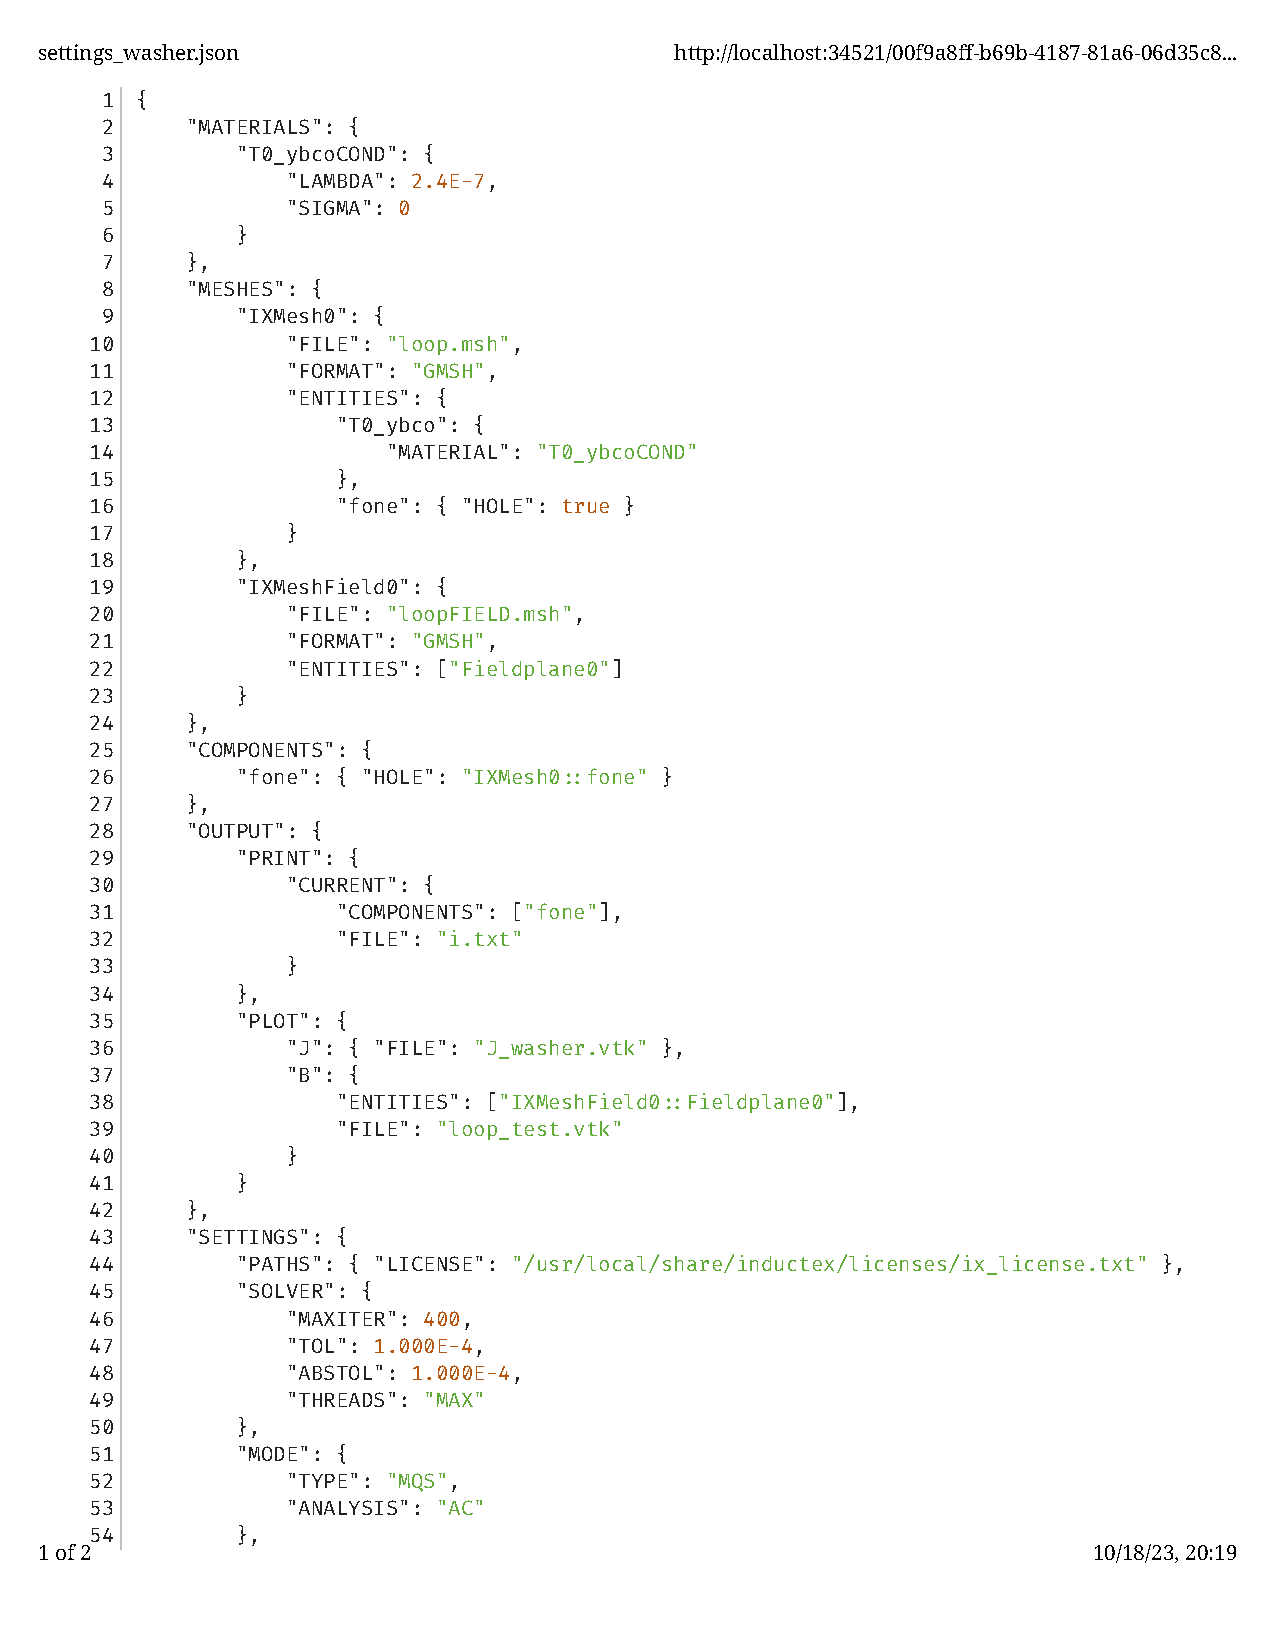
\includegraphics[width=0.9\textwidth]{settings.pdf}
    \label{fig:sett1}
\end{figure}
\newpage
\begin{figure}[H]
    \centering
    \includegraphics[width=0.9\textwidth,page=2]{settings.pdf}
    \label{fig:sett2}
\end{figure}

\chapter{Project Planning Schedule}
\makeatletter\@mkboth{}{Appendix}\makeatother
\label{appen:PPS}

\begin{table}[H]
    \centering
    \begin{tabular}{lll}
        \hline
        \textbf{Task Name}                                   & \textbf{Start Date} & \textbf{Due Date} \\ \hline
        Skripsie Admin                                       & 06/28/2023          & 06/30/2023        \\
        Read Feynmann lectures volume III                    & 07/01/2023          & 07/20/2023        \\
        Read S.M. Anton's PhD thesis                         & 07/21/2023          & 08/07/2023        \\
        Complete and submit GA plan                           & 08/08/2023          & 08/09/2023        \\
        Develop, Implement and test noise extraction module  & 08/10/2023          & 09/03/2023        \\
        Develop, Implement and test mesh optimisation module & 09/04/2023          & 09/23/2023        \\
        Determine Lit review topics                          & 08/10/2023          & 08/12/2023        \\
        Write first 3 sections of lit review                 & 08/13/2023          & 09/02/2023        \\
        write the last three sections of lit review              & 09/03/2023          & 09/23/2023        \\
        write design section                                 & 09/24/2023          & 10/07/2023        \\
        obtain results for results section                   & 09/24/2023          & 10/11/2023        \\
        write results section                                & 10/12/2023          & 10/22/2023        \\
        write introduction                                   & 10/18/2023          & 10/20/2023        \\
        submit preliminary report                            & 10/21/2023          & 10/21/2023        \\
        Make changes to report as recommended by supervisor  & 10/23/2023          & 10/29/2023        \\
        Spelling and grammar checks                          & 10/31/2023          & 10/31/2023        \\
        Write abstract                                       & 10/30/2023          & 10/30/2023        \\
        Create poster and video                              & 11/01/2023          & 11/04/2023        \\
        final check and submission                           & 11/05/2023          & 11/05/2023        \\
        final submission due                                 & 11/05/2023          & 11/06/2023        \\ \hline
        \end{tabular}
        \caption{The project planning schedule}
        \label{tab:pps}
    \end{table}


\chapter{Outcomes Compliance}
\makeatletter\@mkboth{}{Appendix}\makeatother
\label{appen:OC}

\section{GA 1. Problem Solving}
This project required the implementation of an algorithm to calculate the expected noise power in a SQUID. It extends on previous works by generalizing existing techniques to work on any geometry. The algorithm converts a complex 3-dimensional mesh into a single number. The task does not have a defined solution and requires solving many individual problems including but not limited to numerically calculating a surface integral, electromagnetic simulation with TetraHenry, mesh optimisation and modelling of superconducting structures. The details of these challenges are discussed in Chapter \ref{chap:nex} and \ref{chap:meshopt}.

\section{GA 2. Application of Scientific and Engineering Knowledge}
The topic relied on a good understanding of scientific and engineering concepts introduced in my undergraduate years as well as the application of this knowledge to solve open-ended problems. It required knowledge of calculus, vector calculus, electromagnetism, and programming. Along with topics introduced in the undergraduate years, a rudimentary understanding of quantum mechanics and superconductors was needed. Chapters \ref{chap:litreview} and \ref{chap:solutiondevelopment} show the fulfilment of these outcomes.
\section{GA 3. Engineering Design}
The problem statement was very open-ended and required refinement (Chapter \ref{chap:dgoals}). System design techniques were used to solve the engineering design problem in Chapter \ref{chap:high level design}. Once the problem was formally defined it was broken down into smaller sub-problems in Chapter \ref{chap:ddesign}. Solving the sub-problems required drawing knowledge from a wide variety of sources about the topics listed in GA 2.
\section{GA 4. Investigations, experiments and data analysis}
Once the system was implemented an investigation was performed to determine the validity of the results. This required using previous results obtained by simulation as well as physical tests and comparing them to results obtained from my system. The system was tested for accuracy (how closely the output of my system when operating on a previously solved problem matches the true solution) and performance. The testing procedure was designed and then implemented using Python. The regex and OS modules were used to perform parameter sweeps and automate testing. The data output from this testing procedure was analysed to extract conclusions about the performance and accuracy of the system. This achievement of this outcome is demonstrated in Chapter \ref{chap:results}. 
\section{GA 5. Engineering methods, skills and tools, including Information Technology}
To perform the data analysis required as mentioned in GA 4 jupyter notebooks were used in conjunction with the numpy, pandas, matlpotlib and seaborn libraries. The results of this analysis are shown in \ref{chap:results}. Electromagnetic simulations were done with TetraHenry and InductEx. CMake and VCPKG were used to manage compilation and code dependencies. Knowledge of the CLion IDE was crucial to the implementation of this project. GitHub and Git were used for project backup and source control. To model the 3D SQUID structures they had to be created with GMSH. This was done using the GMSH scripting language. Evidence of the above can be found in the GitHub repository \cite{paulcode}. ParaView was used to quickly visualise the results generated by TetraHenry. To improve personal productivity Trello was used to track active tasks as well as future tasks.

\section{GA 6. Professional and technical communication}
The project includes a written report and an oral presentation. These demonstrate competence to communicate effectively, both orally and in writing. Communication with my supervisor included progress reports both as presentations and demonstrations of work progress.

\section{GA 8. Individual work}
I was solely responsible for the completion of my project with little to no input from others. 

\section{GA 9. Independent Learning Ability}
The project required an understanding of complex topics not previously encountered by me. The broad topic gave no context to the required knowledge for the successful completion of the project. Chapter \ref{chap:litreview} demonstrates the process through which I acquired the necessary knowledge. It explores the topics needed to grasp the problem in the order by which they were encountered by me.  

\end{document}

